%\documentclass[tikz, border=5pt]{standalone}
\begin{document}
	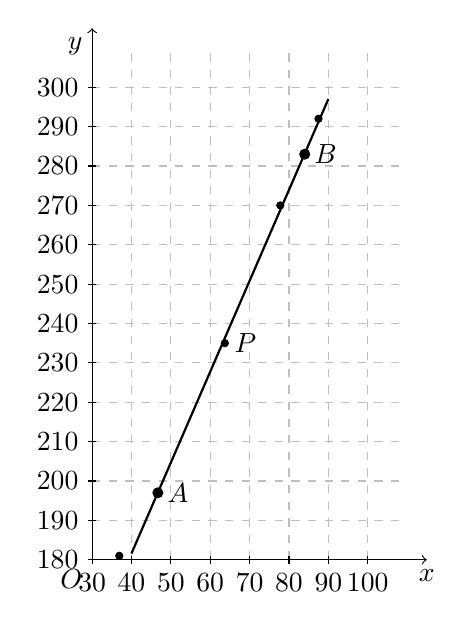
\begin{tikzpicture}[scale=0.5]
		% 2. 绘制网格线(虚线)
		\foreach \x in {0,1,2,...,7} {
			\draw[dashed, gray!50] (\x,0) -- (\x,13);  % 垂直网格线
			% 计算 \x * 10 + 30 并存储到 \result(整数)
			\pgfmathtruncatemacro{\result}{\x * 10 + 30}
			% 绘制刻度短线 + 标注计算后的值
			\draw (\x, 0.1) -- (\x, -0.1) node[below] {$\result$};  % 小竖线(长 0.2 单位)x轴刻度标记 =10x+30
		}
		\foreach \y in {0,1,2,...,12} {
			\draw[dashed, gray!50] (0,\y) -- (8,\y);  % 水平网格线
			\pgfmathtruncatemacro{\result}{\y * 10 + 180}
			\draw (0.1,\y) -- (-0.1,\y) node[left] {$\result$};  % 小竖线(长 0.2 单位)y轴刻度标记
		}
		
		
		% 1. 绘制坐标轴
		\draw[->] (0, 0) -- (8.5, 0) node[below ] {$x$};  % x轴(带箭头和标签)
		\draw[->] (0, 0) -- (0, 13.5) node[below left] {$y$};  % y轴(带箭头和标签)
		\node at (0,0) [below left] {$O$};           % 原点标记
%		\node at (0,0) [below ] {$30$}; 
%		\node at (0,0) [ left] {$180$}; 
		
		
		% 3. 绘制直线(从 (1,0.16) 到 (6,11.7))
		\draw[thick] (1,0.16) -- (6,11.7);
		
		% 4. 标记点 (近似)y≈2.31x−21.5  A(16.7,17) 和 B(54,103)
		\fill (1.67,1.7) circle (4pt) node [ right] {$A$};  % 绘制标注点 A
		\fill (5.4,10.3) circle (4pt) node [ right] {$B$};  % 绘制标注点 B
		\fill (0.69,0.1) circle (3pt) ; 
		\fill (3.37,5.5) circle (3pt) node [ right] {$P$};  % 绘制标注点 P
		\fill (4.78,9) circle (3pt) ;  % 绘制标注点 
		\fill (5.75,11.2) circle (3pt) ;  % 绘制标注点 
		
	\end{tikzpicture}
\end{document}
